\chapter{Reconstruction and Stripping Efficiencies}
\label{chap:apdx_stripeff}

\begin{figure}[htbp]
    \centering
    \begin{subfigure}{\textwidth}
        \centering
        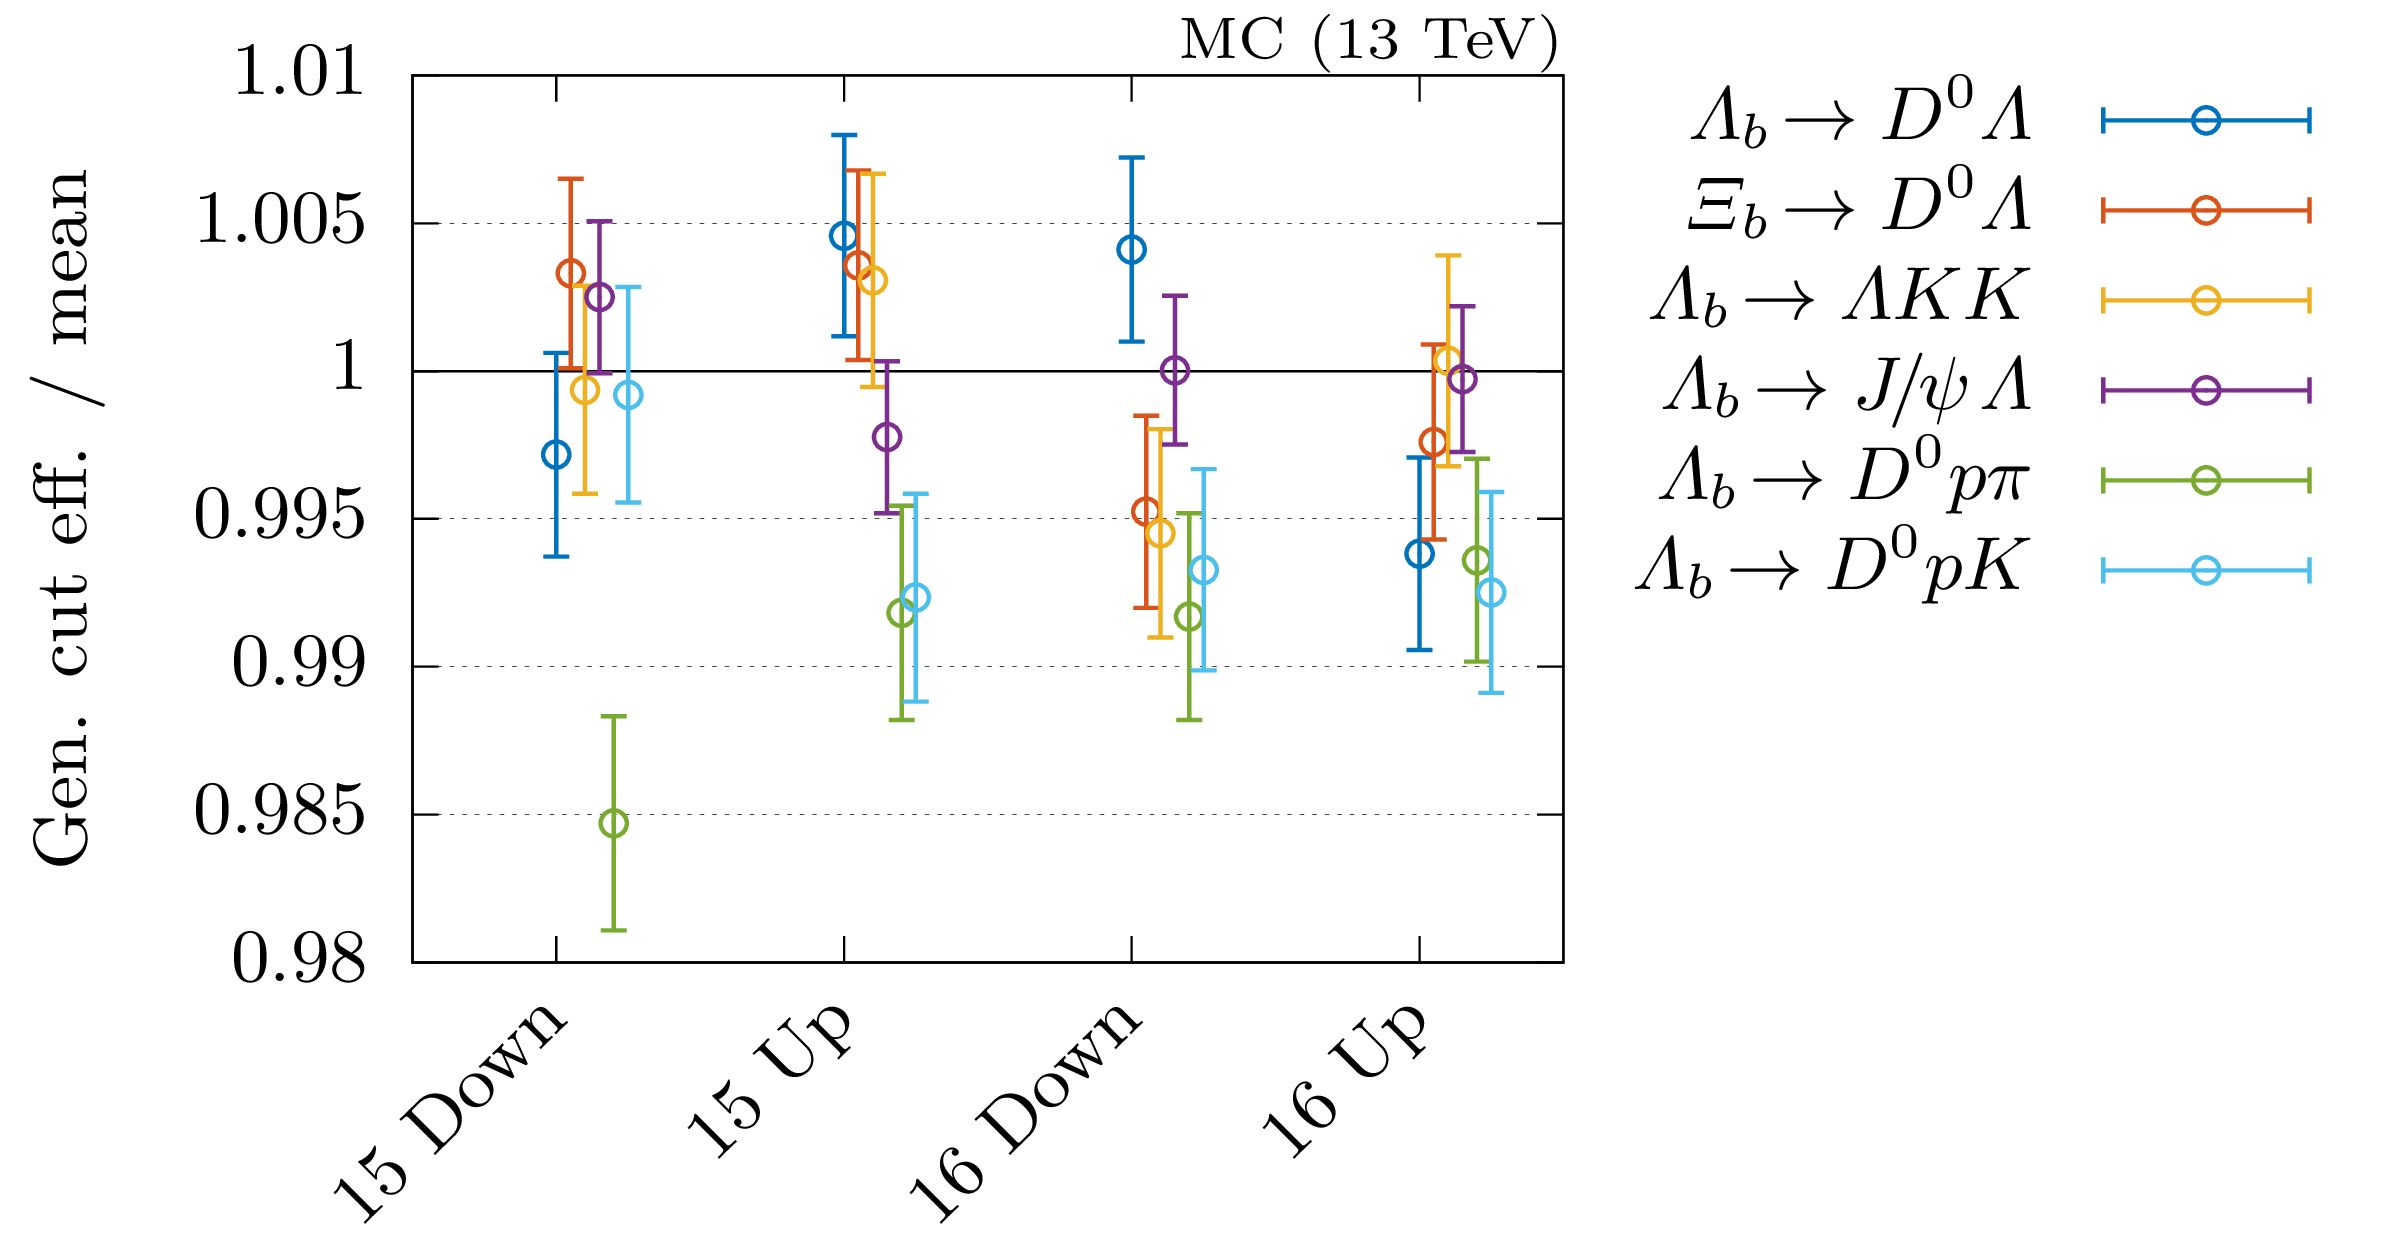
\includegraphics[scale=1.]{stripeff/egeffs1516.png}
    \end{subfigure}
    \par\bigskip 
    \begin{subfigure}{\textwidth}
        \centering
        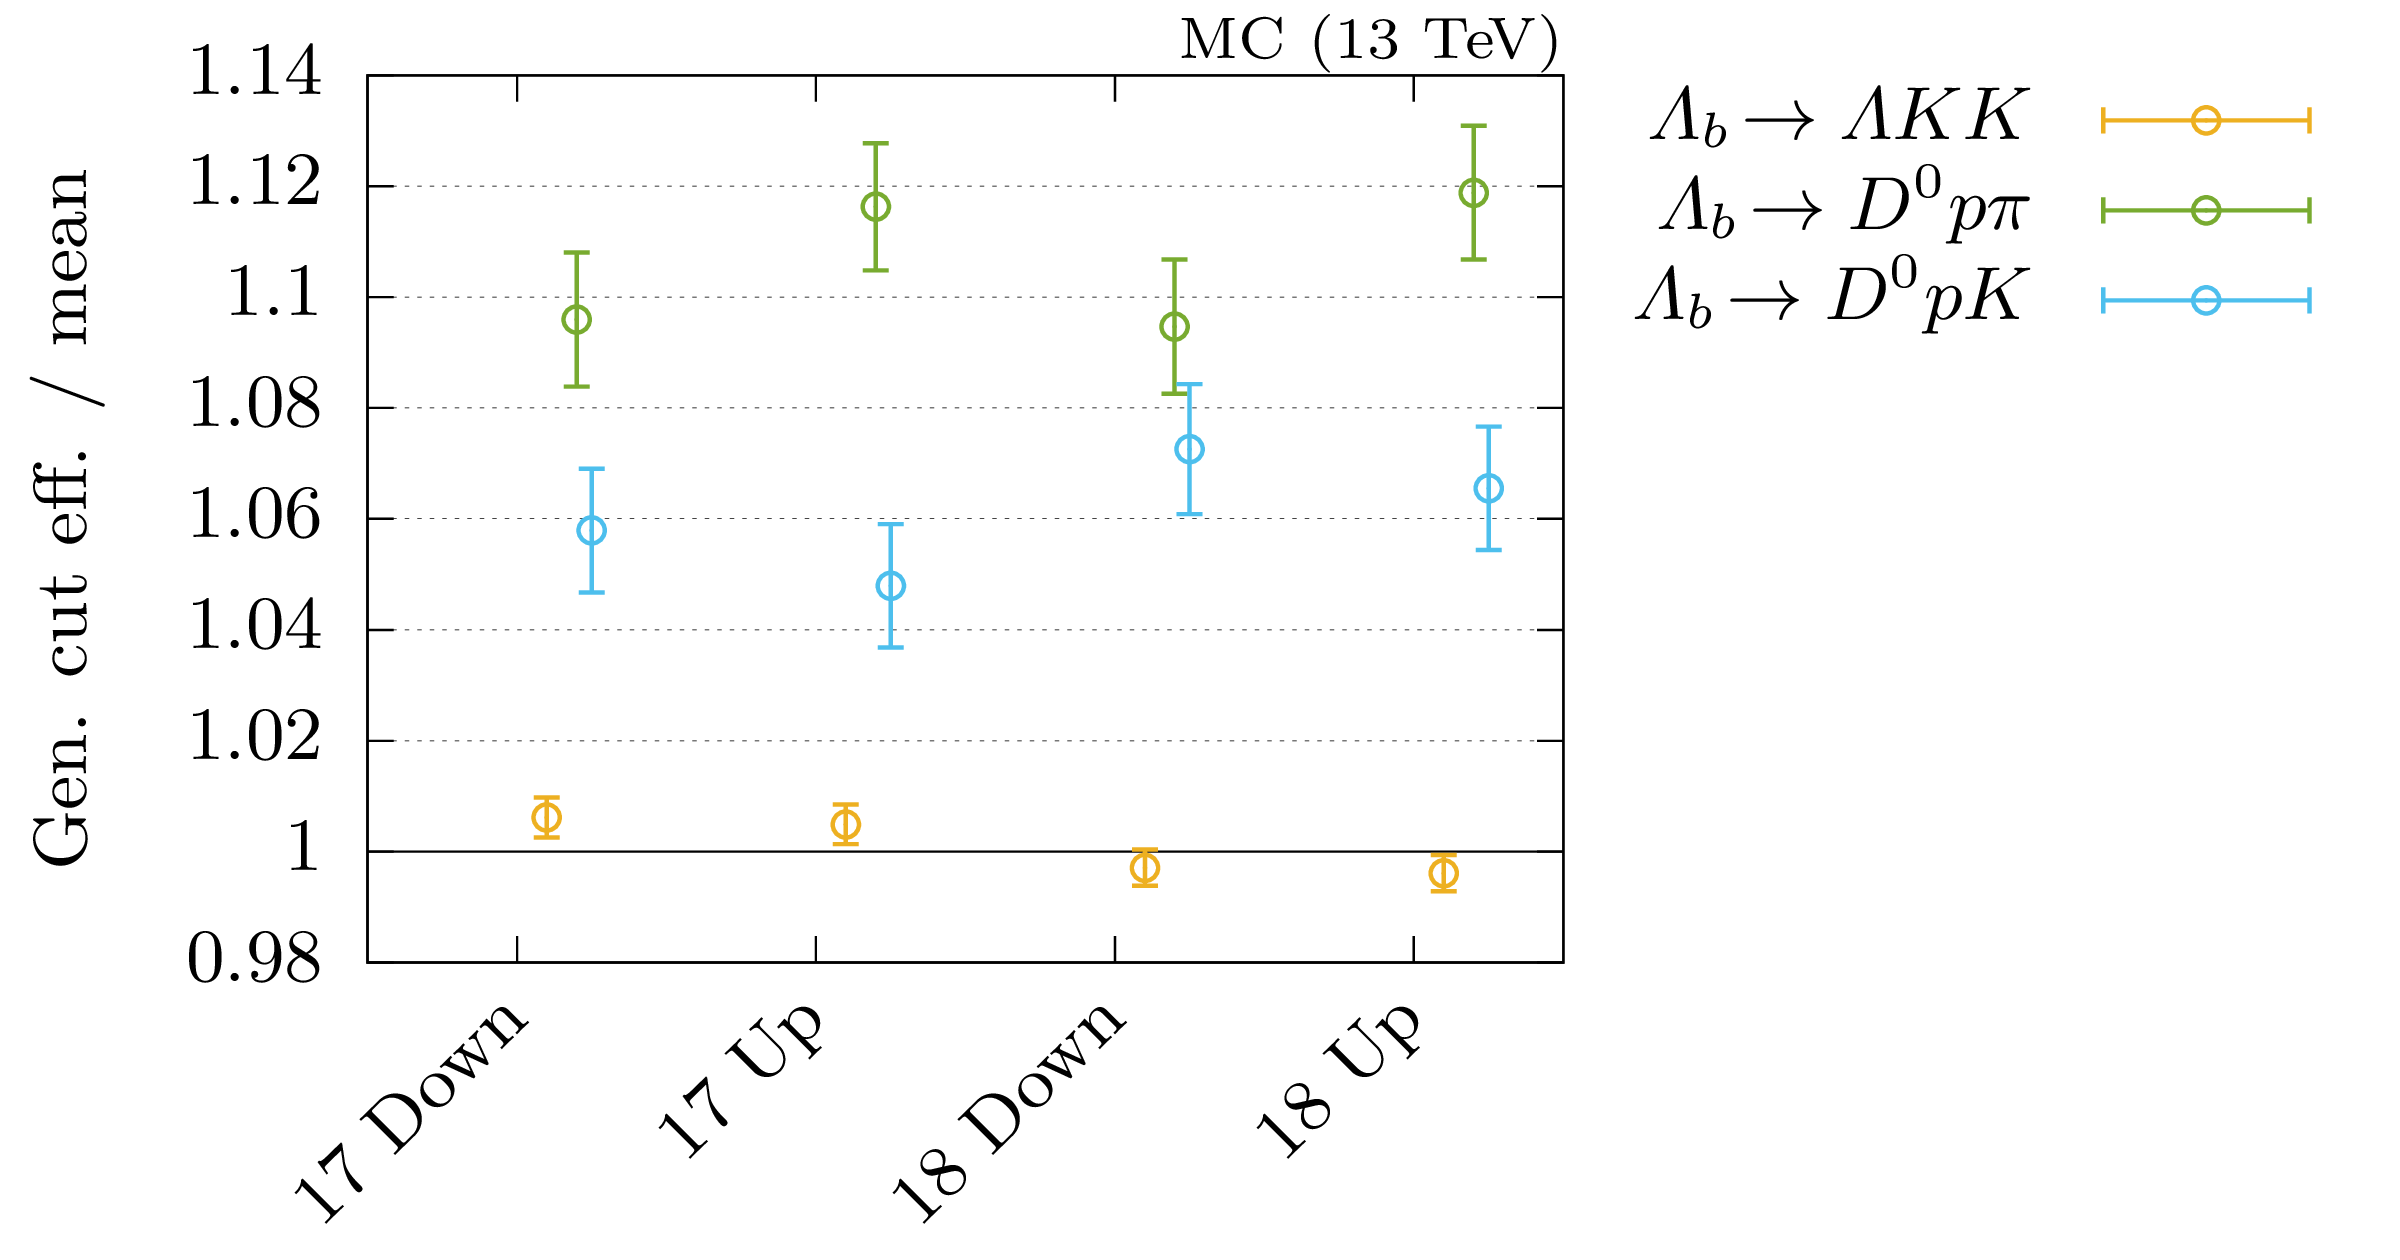
\includegraphics[scale=1.]{stripeff/egeffs1718.png}
    \end{subfigure}
    \caption{Generator cut efficiencies of various decays for different simulation conditions. For the sake of brevity magnet polarities are referred to as \textit{Down} and \textit{Up} for mag.\ down and mag.\ up, respectively. In order to compensate for their wide numerical spread (\cf{}~Tab.~\ref{tab:apdx_simtrig}), each value is normalized to the respective mean of each decay for the full available data set. (Not all decays are simulated for the years 2017 and 2018.)}
    \label{fig:apdx_gencuteff}
\end{figure}

\begin{table}[htbp]
    \centering
    \caption{Simulation and trigger versions, as well as generator cut efficiencies (Gen.\ Cut) and amounts (\#\texttt{DST}) for different decays and simulation conditions. For the sake of brevity, magnet configurations mag.\ down and mag.\ up are abbreviated with $\downarrow$ and $\uparrow$, respectively.}
    \label{tab:apdx_simtrig}
    \begin{tabular}{llllS[separate-uncertainty=false]S[table-format=8.0]}
        \toprule
        Decay & Year & Simulation & Trigger & {Gen. Cut [\%]} & {\#\texttt{DST}} \\
        \midrule
        \midrule
        \decay{\Lb}{\Dz\Lz} & 2015\,$\downarrow$ & \texttt{Sim09c} & \texttt{0x411400a2} & 21.12 \pm 0.07 & 2009840 \\
        & 2015\,$\uparrow$ & \texttt{Sim09c} & \texttt{0x411400a2} & 21.28 \pm 0.07 & 2000794 \\
        & 2016\,$\downarrow$ & \texttt{Sim09c} & \texttt{0x6138160F} & 21.27 \pm 0.07 & 2040356 \\
        & 2016\,$\uparrow$ & \texttt{Sim09c} & \texttt{0x6138160F} & 21.05 \pm 0.07 & 2004574 \\
        \midrule
        \decay{\Xibz}{\Dz\Lz} & 2015\,$\downarrow$ & \texttt{Sim09h} & \texttt{0x411400a2} & 21.29 \pm 0.07 & 1000273 \\
        & 2015\,$\uparrow$ & \texttt{Sim09h} & \texttt{0x411400a2} & 21.29 \pm 0.07 & 1000140 \\
        & 2016\,$\downarrow$ & \texttt{Sim09g} & \texttt{0x6139160F} & 21.12 \pm 0.07 & 3005698 \\
        & 2016\,$\uparrow$ & \texttt{Sim09g} & \texttt{0x6139160F} & 21.17 \pm 0.07 & 3001062 \\
        \midrule
        \decay{\Lb}{\Dz\proton\pim} & 2015\,$\downarrow$ & \texttt{Sim09d} & \texttt{0x411400a2} & 15.50 \pm 0.06 & 151253 \\
        & 2015\,$\uparrow$ & \texttt{Sim09d} & \texttt{0x411400a2} & 15.61 \pm 0.06 & 156266 \\
        & 2016\,$\downarrow$ & \texttt{Sim09d} & \texttt{0x6139160F} & 15.61 \pm 0.06 & 606368 \\
        & 2016\,$\uparrow$ & \texttt{Sim09d} & \texttt{0x6139160F} & 15.64 \pm 0.05 & 604536 \\
        & 2017\,$\downarrow$ & \texttt{Sim09f} & \texttt{0x62661709} & 17.25 \pm 0.19 & 13356991 \\
        & 2017\,$\uparrow$ & \texttt{Sim09f} & \texttt{0x62661709} & 17.57 \pm 0.18 & 13370991 \\
        & 2018\,$\downarrow$ & \texttt{Sim09f} & \texttt{0x617d18a4} & 17.23 \pm 0.19 & 7100997 \\
        & 2018\,$\uparrow$ & \texttt{Sim09f} & \texttt{0x617d18a4} & 17.61 \pm 0.19 & 7621996 \\
        \midrule
        \decay{\Lb}{\Dz\proton\Km} & 2015\,$\downarrow$ & \texttt{Sim09d} & \texttt{0x411400a2} & 17.04 \pm 0.06 & 154815 \\
        & 2015\,$\uparrow$ & \texttt{Sim09d} & \texttt{0x411400a2} & 16.92 \pm 0.06 & 154293 \\
        & 2016\,$\downarrow$ & \texttt{Sim09d} & \texttt{0x6139160F} & 16.94 \pm 0.06 & 607837 \\
        & 2016\,$\uparrow$ & \texttt{Sim09d} & \texttt{0x6139160F} & 16.93 \pm 0.06 & 604865 \\
        & 2017\,$\downarrow$ & \texttt{Sim09f} & \texttt{0x62661709} & 18.04 \pm 0.19 & 13316384 \\
        & 2017\,$\uparrow$ & \texttt{Sim09f} & \texttt{0x62661709} & 17.87 \pm 0.19 & 13857088 \\
        & 2018\,$\downarrow$ & \texttt{Sim09f} & \texttt{0x617d18a4} & 18.29 \pm 0.20 & 7382992 \\
        & 2018\,$\uparrow$ & \texttt{Sim09f} & \texttt{0x617d18a4} & 18.17 \pm 0.19 & 7487998 \\
        \midrule
        \decay{\Lb}{\Lz\Kp\Km} & 2015\,$\downarrow$ & \texttt{Sim09c} & \texttt{0x411400a2} & 22.42 \pm 0.08 & 1002336 \\
        & 2015\,$\uparrow$ & \texttt{Sim09c} & \texttt{0x411400a2} & 22.51 \pm 0.08 & 1004828 \\
        & 2016\,$\downarrow$ & \texttt{Sim09c} & \texttt{0x6138160F} & 22.31 \pm 0.08 & 2502437 \\
        & 2016\,$\uparrow$ & \texttt{Sim09c} & \texttt{0x6138160F} & 22.45 \pm 0.08 & 2500360 \\
        & 2017\,$\downarrow$ & \texttt{Sim09f} & \texttt{0x62661709} & 22.57 \pm 0.08 & 2508342 \\
        & 2017\,$\uparrow$ & \texttt{Sim09f} & \texttt{0x62661709} & 22.55 \pm 0.08 & 2503107 \\
        & 2018\,$\downarrow$ & \texttt{Sim09f} & \texttt{0x617d18a4} & 22.37 \pm 0.07 & 2501960 \\
        & 2018\,$\uparrow$ & \texttt{Sim09f} & \texttt{0x617d18a4} & 22.35 \pm 0.07 & 2504022 \\
        \midrule
        \decay{\Lb}{\jpsi\Lz} & 2015\,$\downarrow$ & \texttt{Sim09c} & \texttt{0x411400a2} & 19.89 \pm 0.05 & 519498 \\
        & 2015\,$\uparrow$ & \texttt{Sim09c} & \texttt{0x411400a2} & 19.79 \pm 0.05 & 506398 \\
        & 2016\,$\downarrow$ & \texttt{Sim09c} & \texttt{0x6139160F} & 19.84 \pm 0.05 & 2008494 \\
        & 2016\,$\uparrow$ & \texttt{Sim09c} & \texttt{0x6139160F} & 19.83 \pm 0.05 & 2008422 \\
        \bottomrule
    \end{tabular}
\end{table}

\begin{sidewaystable}[htbp]
    \centering
    \caption{Total amounts (\#\texttt{DTT}) and product of generator cut efficiency and fractions (\#\texttt{DTT} over \#\texttt{DST}) in percent for different decays (Gen.\ Decay) and data taking condition when reconstructed in the given decay mode (Rec.\ Decay). For the sake of brevity, magnet configurations mag.\ down and mag.\ up are abbreviated with $\downarrow$ and $\uparrow$, respectively. (Part 1/2)}
    \label{tab:apdx_ndstdtt1}
    \begin{tabular}{lllS[table-format=6.0]S[separate-uncertainty=false]S[table-format=6.0]S[separate-uncertainty=false]}
        \toprule
        &&& \multicolumn{2}{c}{{\gls{LL}}} & \multicolumn{2}{c}{{\gls{DD}}} \\
        Gen.\ Decay & Rec.\ Decay & Year & {\#\texttt{DTT}} & {\% \texttt{DTT}} & {\#\texttt{DTT}} & {\% \texttt{DTT}} \\
        \midrule
        \midrule
        \decay{\Lb}{\Dz\Lz} & \decay{\Lb}{\Dz\Lz} & 2015\,$\uparrow$ & 3572 & 0.0375 \pm 0.0006 & 8361 & 0.0879 \pm 0.0010 \\
        && 2015\,$\downarrow$ & 3540 & 0.0377 \pm 0.0006 & 8350 & 0.0888 \pm 0.0010 \\
        && 2016\,$\uparrow$ & 4399 & 0.0459 \pm 0.0007 & 9793 & 0.1021 \pm 0.0011 \\
        && 2016\,$\downarrow$ & 4252 & 0.0447 \pm 0.0007 & 9482 & 0.0996 \pm 0.0011 \\
        \midrule
        \decay{\Xibz}{\Dz\Lz} & \decay{\Lb}{\Dz\Lz} & 2015\,$\uparrow$ & 1980 & 0.0421 \pm 0.0010 & 4813 & 0.1024 \pm 0.0015 \\
        && 2015\,$\downarrow$ & 1953 & 0.0416 \pm 0.0009 & 4692 & 0.0999 \pm 0.0015 \\
        && 2016\,$\uparrow$ & 6984 & 0.0491 \pm 0.0006 & 16126 & 0.1133 \pm 0.0010 \\
        && 2016\,$\downarrow$ & 6918 & 0.0488 \pm 0.0006 & 16227 & 0.1144 \pm 0.0010 \\
        \midrule
        \decay{\Lb}{\Dz\proton\pim} & \decay{\Lb}{\Dz\proton\pim} & 2015\,$\uparrow$ & 7045 & 0.722 \pm 0.009 & {--} & {--} \\
        && 2015\,$\downarrow$ & 7302 & 0.729 \pm 0.009 & {--} & {--} \\
        && 2016\,$\uparrow$ & 32373 & 0.833 \pm 0.005 & {--} & {--} \\
        && 2016\,$\downarrow$ & 31933 & 0.826 \pm 0.005 & {--} & {--} \\
        && 2017\,$\uparrow$ & 692296 & 0.894 \pm 0.010 & {--} & {--} \\
        && 2017\,$\downarrow$ & 696910 & 0.916 \pm 0.009 & {--} & {--} \\
        && 2018\,$\uparrow$ & 339065 & 0.823 \pm 0.009 & {--} & {--} \\
        && 2018\,$\downarrow$ & 355522 & 0.821 \pm 0.009 & {--} & {--} \\
        \midrule
        \decay{\Lb}{\Dz\proton\Km} & \decay{\Lb}{\Dz\proton\Km} & 2015\,$\uparrow$ & 6850 & 0.754 \pm 0.009 & {--} & {--} \\
        && 2015\,$\downarrow$ & 6908 & 0.758 \pm 0.009 & {--} & {--} \\
        && 2016\,$\uparrow$ & 30117 & 0.839 \pm 0.006 & {--} & {--} \\
        && 2016\,$\downarrow$ & 30247 & 0.846 \pm 0.006 & {--} & {--} \\
        && 2017\,$\uparrow$ & 690195 & 0.935 \pm 0.010 & {--} & {--} \\
        && 2017\,$\downarrow$ & 716056 & 0.923 \pm 0.010 & {--} & {--} \\
        && 2018\,$\uparrow$ & 346474 & 0.858 \pm 0.009 & {--} & {--} \\
        && 2018\,$\downarrow$ & 346040 & 0.840 \pm 0.009 & {--} & {--} \\
        \bottomrule
    \end{tabular}
\end{sidewaystable}

\begin{sidewaystable}[htbp]
    \centering
    \caption{Total amounts (\#\texttt{DTT}) and product of generator cut efficiency and fractions (\#\texttt{DTT} over \#\texttt{DST}) in percent for different decays (Gen.\ Decay) and data taking condition when reconstructed in the given decay mode (Rec.\ Decay). For the sake of brevity, magnet configurations mag.\ down and mag.\ up are abbreviated with $\downarrow$ and $\uparrow$, respectively. (Part 2/2)}
    \label{tab:apdx_ndstdtt2}
    \begin{tabular}{lllS[table-format=6.0]S[separate-uncertainty=false]S[table-format=6.0]S[separate-uncertainty=false]}
        \toprule
        &&& \multicolumn{2}{c}{{\gls{LL}}} & \multicolumn{2}{c}{{\gls{DD}}} \\
        Gen.\ Decay & Rec.\ Decay & Year & {\#\texttt{DTT}} & {\% \texttt{DTT}} & {\#\texttt{DTT}} & {\% \texttt{DTT}} \\
        \midrule
        \midrule
        \midrule
        \decay{\Lb}{\Dz\proton\pim} & \decay{\Lb}{\Dz\Lz} & 2015\,$\uparrow$ & 309 & 0.0317 \pm 0.0018 & {--} & {--} \\
        && 2015\,$\downarrow$ & 334 & 0.0334 \pm 0.0018 & {--} & {--} \\
        && 2016\,$\uparrow$ & 1283 & 0.0330 \pm 0.0009 & {--} & {--} \\
        && 2016\,$\downarrow$ & 1289 & 0.0333 \pm 0.0009 & {--} & {--} \\
        \midrule
        \decay{\Lb}{\Dz\Kp\Km} & \decay{\Lb}{\Dz\Kp\Km} & 2015\,$\uparrow$ & 4870 & 0.1089 \pm 0.0016 & 17622 & 0.3942 \pm 0.0033 \\
        && 2015\,$\downarrow$ & 4881 & 0.1093 \pm 0.0016 & 17648 & 0.3953 \pm 0.0033 \\
        && 2016\,$\uparrow$ & 12903 & 0.1151 \pm 0.0011 & 43827 & 0.3908 \pm 0.0023 \\
        && 2016\,$\downarrow$ & 12865 & 0.1155 \pm 0.0011 & 44038 & 0.3953 \pm 0.0023 \\
        && 2017\,$\uparrow$ & 13463 & 0.1212 \pm 0.0011 & 48639 & 0.4377 \pm 0.0025 \\
        && 2017\,$\downarrow$ & 13322 & 0.1200 \pm 0.0011 & 48581 & 0.4376 \pm 0.0025 \\
        && 2018\,$\uparrow$ & 13339 & 0.1193 \pm 0.0011 & 48118 & 0.4303 \pm 0.0024 \\
        && 2018\,$\downarrow$ & 13407 & 0.1197 \pm 0.0011 & 48428 & 0.4323 \pm 0.0024 \\
        \midrule
        \decay{\Lb}{\Dz\Kp\Km} & \decay{\Lb}{\Dz\Lz} & 2015\,$\uparrow$ & 165 & 0.00369 \pm 0.00029 & 443 & 0.0099 \pm 0.0005 \\
        && 2015\,$\downarrow$ & 157 & 0.00352 \pm 0.00028 & 397 & 0.0089 \pm 0.0004 \\
        && 2016\,$\uparrow$ & 435 & 0.00388 \pm 0.00019 & 1084 & 0.00967 \pm 0.00030 \\
        && 2016\,$\downarrow$ & 429 & 0.00385 \pm 0.00019 & 829 & 0.00744 \pm 0.00026 \\
        && 2017\,$\uparrow$ & 408 & 0.00367 \pm 0.00018 & 1088 & 0.00979 \pm 0.00030 \\ 
        && 2017\,$\downarrow$ & 442 & 0.00398 \pm 0.00019 & 961 & 0.00866 \pm 0.00028 \\
        && 2018\,$\uparrow$ & 418 & 0.00374 \pm 0.00018 & 1091 & 0.00976 \pm 0.00030 \\
        && 2018\,$\downarrow$ & 421 & 0.00376 \pm 0.00018 & 1162 & 0.01037 \pm 0.00031 \\
        \midrule
        \decay{\Lb}{\jpsi\Lz} & \decay{\Lb}{\jpsi\Lz} & 2015\,$\uparrow$ & 4072 & 0.1559 \pm 0.0025 & 14344 & 0.549 \pm 0.005 \\
        && 2015\,$\downarrow$ & 3989 & 0.1559 \pm 0.0025 & 13870 & 0.542 \pm 0.005 \\
        && 2016\,$\uparrow$ & 16537 & 0.1633 \pm 0.0013 & 55604 & 0.5492 \pm 0.0027 \\
        && 2016\,$\downarrow$ & 16731 & 0.1652 \pm 0.0013 & 55387 & 0.5469 \pm 0.0027 \\
        \bottomrule
    \end{tabular}
\end{sidewaystable}
